% Options for packages loaded elsewhere
\PassOptionsToPackage{unicode}{hyperref}
\PassOptionsToPackage{hyphens}{url}
\PassOptionsToPackage{dvipsnames,svgnames,x11names}{xcolor}
\documentclass[
  brazilian,
  12pt,
  a4paper,
]{article}
\usepackage{xcolor}
\usepackage[margin=1in]{geometry}
\usepackage{amsmath,amssymb}
\setcounter{secnumdepth}{-\maxdimen} % remove section numbering
\usepackage{iftex}
\ifPDFTeX
  \usepackage[T1]{fontenc}
  \usepackage[utf8]{inputenc}
  \usepackage{textcomp} % provide euro and other symbols
\else % if luatex or xetex
  \usepackage{unicode-math} % this also loads fontspec
  \defaultfontfeatures{Scale=MatchLowercase}
  \defaultfontfeatures[\rmfamily]{Ligatures=TeX,Scale=1}
\fi
\usepackage{lmodern}
\ifPDFTeX\else
  % xetex/luatex font selection
\fi
% Use upquote if available, for straight quotes in verbatim environments
\IfFileExists{upquote.sty}{\usepackage{upquote}}{}
\IfFileExists{microtype.sty}{% use microtype if available
  \usepackage[]{microtype}
  \UseMicrotypeSet[protrusion]{basicmath} % disable protrusion for tt fonts
}{}
\makeatletter
\@ifundefined{KOMAClassName}{% if non-KOMA class
  \IfFileExists{parskip.sty}{%
    \usepackage{parskip}
  }{% else
    \setlength{\parindent}{0pt}
    \setlength{\parskip}{6pt plus 2pt minus 1pt}}
}{% if KOMA class
  \KOMAoptions{parskip=half}}
\makeatother
\usepackage{longtable,booktabs,array}
\usepackage{caption}
\captionsetup[table]{skip=6pt}
\newcounter{none} % for unnumbered tables
\usepackage{calc} % for calculating minipage widths
% Correct order of tables after \paragraph or \subparagraph
\usepackage{etoolbox}
\makeatletter
\patchcmd\longtable{\par}{\if@noskipsec\mbox{}\fi\par}{}{}
\makeatother
\ifLuaTeX
\usepackage[bidi=basic,shorthands=off]{babel}
\else
\usepackage[bidi=default,shorthands=off]{babel}
\fi
\ifLuaTeX
  \usepackage{selnolig} % disable illegal ligatures
\fi
\setlength{\emergencystretch}{3em} % prevent overfull lines
\providecommand{\tightlist}{%
  \setlength{\itemsep}{0pt}\setlength{\parskip}{0pt}}

\usepackage{caption}
\usepackage{graphicx}
\usepackage{pdflscape}
\usepackage{etoolbox}
\usepackage{fancyvrb}
\fvset{fontsize=\small}
\AtBeginEnvironment{longtable}{\footnotesize}
\setlength{\emergencystretch}{3em}
\setlength{\parskip}{0.4em}
\AtBeginDocument{\def\UrlBreaks{\do\_\do\/\do\.\do\-}\Urlmuskip=0mu}
\usepackage{bookmark}
\IfFileExists{xurl.sty}{\usepackage{xurl}}{} % add URL line breaks if available
\urlstyle{same}
% fallback for those not using the hyperref driver hyperxmp:
\makeatletter
\@ifundefined{xmpquote}{\newcommand{\xmpquote}[1]{#1}}{}
\makeatother
\hypersetup{
  pdftitle={Modelo Entidade-Relacionamento da Aplicação UnB RU},
  pdflang={pt-BR},
  colorlinks=true,
  linkcolor={black},
  filecolor={Maroon},
  citecolor={Blue},
  urlcolor={blue},
  pdfcreator={LaTeX via pandoc}}

\title{Modelo Entidade-Relacionamento da Aplicação UnB RU}
\usepackage{etoolbox}
\makeatletter
\providecommand{\subtitle}[1]{% add subtitle to \maketitle
  \apptocmd{\@title}{\par {\large #1 \par}}{}{}
}
\makeatother
\subtitle{Sprint 1 --- Segunda etapa}
\author{}
\date{23 de outubro de 2026}

\begin{document}
\maketitle

{
\setcounter{tocdepth}{2}
\tableofcontents
}
\section{Introdução}\label{introduuxe7uxe3o}

O UnB RU é um sistema de gerenciamento do Restaurante Universitário da
Universidade de Brasília. O domínio reúne a conta do estudante, a compra
de créditos, a operação de catracas, a gestão de restaurantes, a
consulta de cardápios e a produção de relatórios para estudantes e
administradores. Este relatório apresenta um modelo
entidade-relacionamento lógico, com indicação de chaves e restrições
para sua futura implementação em Ruby on Rails e banco relacional.

O documento segue as seções do template \path|ER-MyRottenPotatoes.tex|,
disponibilizado em \path|TemplateRelatorioSprint1_1|: Introdução,
Entidades Principais, Modelo Relacional UML e Considerações Finais. O
diagrama utiliza a notação ER de pé de galinha, em vez da notação de
classes UML do exemplo, conforme a possibilidade de utilizar Mermaid
indicada no enunciado. O apêndice registra o uso de inteligência
artificial na elaboração.

{\def\LTcaptype{none} % do not increment counter
\begin{longtable}[]{@{}lll@{}}
\toprule\noalign{}
Integrante & Matrícula & Papel na sprint \\
\midrule\noalign{}
\endhead
\bottomrule\noalign{}
\endlastfoot
Daniel Dezan Baby & 232046097 & Scrum Master \\
Leonardo Tome Sampaio & 222005448 & Product Owner \\
Luis Eduardo Curi Serra & 251033574 & Desenvolvedor \\
Tarsila Marques de Oliveira Alves & 242012029 & Desenvolvedora \\
Weldo Gonçalves da Silva Junior & 222014133 & Desenvolvedor \\
\end{longtable}
}

\textbf{Base de requisitos.} Foram analisados os 12 arquivos em
\texttt{features/}, a wiki do projeto, o arquivo \texttt{cardapio.json}
e o enunciado \texttt{sprint1.pdf}. As referências F01 a F12
correspondem à numeração utilizada na wiki. O relatório descreve uma
proposta de modelagem: as tabelas e os serviços aqui especificados ainda
não constituem uma aplicação implementada.

\textbf{Limites e premissas.} Os requisitos especificam comportamentos,
mas não resolvem todas as decisões de persistência. A separação de
perfis, a política de consumo de créditos, o armazenamento de auditoria
de exportações e o tratamento de concorrência são decisões propostas
neste relatório e identificadas como tais. Os preços presentes nos
cenários são dados de teste; o modelo mantém tarifas e valores
históricos, sem escolher uma tarifa definitiva.

\section{Entidades Principais}\label{entidades-principais}

\subsection{Convenções do modelo}\label{convenuxe7uxf5es-do-modelo}

Todas as entidades possuem \texttt{id} como chave primária do tipo
\texttt{bigint}, exceto \texttt{UsuarioPapel}, cuja chave é o par de
chaves estrangeiras. O sufixo \texttt{\_id} identifica uma FK. As
tabelas recebem os campos técnicos \texttt{created\_at} e
\texttt{updated\_at} quando aplicáveis; eles não substituem os horários
de negócio, como confirmação do pagamento e passagem na catraca.

Valores monetários usam \texttt{decimal(12,2)}, nunca ponto flutuante.
Matrículas e identificações são textos, preservando zeros à esquerda.
Datas e horas de eventos são armazenadas com referência temporal
inequívoca em UTC e exibidas no fuso \path|America/Sao_Paulo|.
Intervalos de datas do usuário incluem o primeiro e o último dia; sua
consulta utiliza o início do primeiro dia até, sem incluir, o início do
dia posterior ao último.

Nos atributos abaixo, \textbf{obrigatório} significa \texttt{NOT\ NULL};
\textbf{opcional} significa que \texttt{NULL} é permitido. A descrição
de uma unicidade composta aplica-se à combinação dos campos. As
entidades de apoio ampliam o modelo para atender aos cenários de erro e
à auditoria, além dos fluxos felizes.

\subsection{1. Usuario --- identidade e
credenciais}\label{usuario-identidade-e-credenciais}

Centraliza os dados de autenticação de estudantes, funcionários e
administradores, evitando credenciais duplicadas para uma pessoa com
mais de um perfil.

\begin{itemize}
\tightlist
\item
  \texttt{id}: PK.
\item
  \texttt{nome}: texto obrigatório, utilizado na identificação de
  relatórios e da conta.
\item
  \texttt{identificacao}: texto obrigatório e único; login de
  funcionário sem impor formato numérico, conforme F04.
\item
  \texttt{email}: texto obrigatório, normalizado e único sem diferenciar
  maiúsculas de minúsculas.
\item
  \texttt{password\_digest}: texto obrigatório contendo o hash da senha;
  a senha em texto não é persistida.
\item
  \texttt{ativo}: booleano obrigatório; conta inativa não cria uma
  sessão válida.
\end{itemize}

\textbf{Relacionamentos:} um usuário possui zero ou um cadastro de
estudante, zero ou muitas sessões, zero ou muitas emissões de relatório
e um ou mais papéis associados após a conclusão do cadastro.

\textbf{Regras atendidas:} F01 e F04. O cadastro público cria somente o
papel de estudante. A validação de domínio institucional aplica-se ao
cadastro estudantil, sem inventar uma exigência equivalente para
funcionários. O conjunto exato de domínios aceitos e a consulta que
confirma vínculo ativo com a UnB precisam ser definidos pela equipe.

\subsection{2. Papel --- permissões por
perfil}\label{papel-permissuxf5es-por-perfil}

\begin{itemize}
\tightlist
\item
  \texttt{id}: PK.
\item
  \texttt{codigo}: texto obrigatório e único, com os valores propostos
  \texttt{estudante}, \texttt{funcionario}, \texttt{administrador} e
  \path|administrador_geral|.
\item
  \texttt{descricao}: texto obrigatório que explica o conjunto de
  permissões.
\end{itemize}

\textbf{Relacionamento:} um papel pode estar associado a nenhum ou
muitos usuários por \texttt{UsuarioPapel}.

\textbf{Decisão proposta:} permitir múltiplos papéis evita interpretar
uma conta exclusivamente estudantil como conta de funcionário. O
administrador geral pode consultar o relatório administrativo e tem a
permissão específica de F12. A atribuição de papéis é administrativa e
não pode ser recebida do formulário de cadastro público.

\subsection{3. UsuarioPapel --- associação de
autorização}\label{usuariopapel-associauxe7uxe3o-de-autorizauxe7uxe3o}

\begin{itemize}
\tightlist
\item
  \texttt{usuario\_id}: FK obrigatória para \texttt{Usuario}.
\item
  \texttt{papel\_id}: FK obrigatória para \texttt{Papel}.
\item
  Chave primária composta por \texttt{(usuario\_id,\ papel\_id)}.
\end{itemize}

\textbf{Relacionamento:} resolve a associação N:N entre usuários e
papéis, impedindo a atribuição duplicada do mesmo papel. A existência do
cadastro de estudante deve ser coerente com o papel estudantil.

\subsection{4. Estudante --- vínculo universitário e
conta}\label{estudante-vuxednculo-universituxe1rio-e-conta}

\begin{itemize}
\tightlist
\item
  \texttt{id}: PK.
\item
  \texttt{usuario\_id}: FK obrigatória e única para \texttt{Usuario}.
\item
  \texttt{matricula}: texto obrigatório e único, com exatamente nove
  dígitos.
\item
  \texttt{vinculo\_ativo}: booleano obrigatório, resultante da validação
  do vínculo universitário.
\end{itemize}

\textbf{Relacionamentos:} cada estudante pertence a um usuário e pode
possuir muitas recargas, leituras de identificação e movimentações
financeiras.

\textbf{Saldo:} é calculado pela soma dos valores assinados de
\path|MovimentacaoSaldo|. Uma conta nova tem saldo zero. Não existe uma
segunda coluna de saldo independente neste modelo; uma futura otimização
com saldo armazenado deve manter reconciliação com o extrato. Isso evita
atualizar o saldo por uma cobrança ainda pendente.

\subsection{5. SessaoAutenticacao --- validade do
acesso}\label{sessaoautenticacao-validade-do-acesso}

\begin{itemize}
\tightlist
\item
  \texttt{id}: PK; \texttt{usuario\_id}: FK obrigatória para
  \texttt{Usuario}.
\item
  \texttt{token\_digest}: texto obrigatório e único, representando um
  identificador de sessão sem armazenar o token utilizável.
\item
  \texttt{autenticada\_em} e \texttt{expira\_em}: instantes
  obrigatórios, com expiração posterior à autenticação.
\item
  \texttt{encerrada\_em}: instante opcional; preenchido em logout ou
  revogação.
\item
  \path|ponto_acesso_pendente|: booleano obrigatório, inicialmente
  verdadeiro na aplicação de controle.
\end{itemize}

\textbf{Relacionamentos:} uma sessão pertence a um usuário e possui zero
ou muitas configurações confirmadas de ponto de acesso. Somente uma
configuração pode estar vigente por sessão.

\textbf{Regras atendidas:} F04 e F05. Uma sessão é válida se não foi
encerrada, não expirou e o usuário permanece ativo. O prazo de expiração
não foi definido pelos cenários e permanece configurável. A
reconfiguração pendente bloqueia operações mesmo que a configuração
anterior ainda exista para auditoria.

\subsection{6. ConfiguracaoPontoAcesso --- contexto confirmado de
operação}\label{configuracaopontoacesso-contexto-confirmado-de-operauxe7uxe3o}

\begin{itemize}
\tightlist
\item
  \texttt{id}: PK; \path|sessao_autenticacao_id|: FK obrigatória para
  \path|SessaoAutenticacao|.
\item
  \texttt{catraca\_id}: FK obrigatória para \texttt{Catraca}.
\item
  \texttt{confirmada\_em}: instante obrigatório da confirmação válida.
\item
  \texttt{finalizada\_em}: instante opcional; quando preenchido, deve
  ser posterior ou igual à confirmação.
\end{itemize}

\textbf{Relacionamentos:} cada configuração pertence a uma sessão e a
uma catraca; pode originar muitos registros de acesso. O funcionário é
obtido pela sessão; o restaurante, pela catraca e seu piso.

\textbf{Regras atendidas:} F05 e F07. A escolha feita no formulário
ainda não é uma configuração confirmada. Uma troca válida finaliza a
configuração anterior e cria outra, sem reatribuir acessos antigos. Uma
tentativa inválida não cria configuração nem substitui a anterior.
Logout ou expiração tornam o contexto inutilizável, preservando seus
registros de auditoria.

\subsection{7. UnidadeGestora --- agrupamento
administrativo}\label{unidadegestora-agrupamento-administrativo}

\begin{itemize}
\tightlist
\item
  \texttt{id}: PK.
\item
  \texttt{nome}: texto obrigatório e único.
\item
  \texttt{ativa}: booleano obrigatório.
\end{itemize}

\textbf{Relacionamento:} uma unidade gestora possui zero ou muitos
restaurantes; cada restaurante pertence a exatamente uma unidade.
Permite o filtro de F09. ``Campus Darcy Ribeiro'' é a unidade padrão
prevista na feature, identificada por cadastro, sem fixar seu ID no
código.

\subsection{8. Restaurante --- unidade de
atendimento}\label{restaurante-unidade-de-atendimento}

\begin{itemize}
\tightlist
\item
  \texttt{id}: PK; \path|unidade_gestora_id|: FK obrigatória para
  \texttt{UnidadeGestora}.
\item
  \texttt{nome}: texto obrigatório, único no sistema segundo a validação
  de nome existente de F08.
\item
  \texttt{numero}: inteiro obrigatório, positivo e único na unidade
  gestora; determina a ordenação de F09.
\item
  \path|capacidade_refeicoes_hora|: inteiro obrigatório e maior que
  zero.
\item
  \texttt{ativo}: booleano obrigatório.
\end{itemize}

\textbf{Relacionamentos:} cada restaurante possui um ou muitos pisos e
zero ou muitos serviços de refeição. A quantidade de pisos é obtida
pelos seus registros, evitando mantê-la duplicada.

\textbf{Regras atendidas:} F05, F08 e F09. A criação dos pisos e do
restaurante é atômica. Não se pode remover um restaurante com catracas
associadas; vínculos históricos também impedem exclusão física. Para
cadastros com histórico, a proposta é desativar e preservar as
referências. Essa política complementa os cenários e deve ser validada
pelo grupo.

\subsection{9. Piso --- localização
física}\label{piso-localizauxe7uxe3o-fuxedsica}

\begin{itemize}
\tightlist
\item
  \texttt{id}: PK; \texttt{restaurante\_id}: FK obrigatória para
  \texttt{Restaurante}.
\item
  \texttt{numero}: inteiro obrigatório e positivo.
\item
  Unicidade composta \texttt{(restaurante\_id,\ numero)}.
\end{itemize}

\textbf{Relacionamento:} um piso pertence a um restaurante e pode
possuir zero ou muitas catracas. A seleção de um piso inexistente é
rejeitada em F08. O piso não muda de restaurante depois de ser
referenciado por uma catraca com histórico.

\subsection{10. Catraca --- equipamento de
controle}\label{catraca-equipamento-de-controle}

\begin{itemize}
\tightlist
\item
  \texttt{id}: PK; \texttt{piso\_id}: FK obrigatória para \texttt{Piso}.
\item
  \texttt{identificacao}: texto obrigatório, como ``Catraca 01'' ou
  ``CAT-01''.
\item
  \texttt{ativa}: booleano obrigatório; permite desativação
  administrativa.
\item
  \texttt{online}: booleano obrigatório; representa o estado operacional
  conhecido.
\item
  \path|estado_verificado_em|: instante opcional da última verificação
  de conectividade.
\end{itemize}

\textbf{Relacionamentos:} cada catraca pertence a um piso e pode
participar de muitas configurações de ponto de acesso. Os acessos
históricos são encontrados pelas configurações.

\textbf{Unicidade:} a identificação é única por restaurante, inclusive
entre pisos distintos. Uma validação de serviço deve consultar o
restaurante do piso; em PostgreSQL, a garantia concorrente pode usar um
gatilho que serialize cadastros pela linha do restaurante. Um índice
apenas em \texttt{(piso\_id,\ identificacao)} seria insuficiente para o
cenário de identificação repetida em outro piso do mesmo restaurante.

\textbf{Regras atendidas:} F05, F07, F08 e F09. \texttt{ativa} e
\texttt{online} representam conceitos distintos. Uma catraca em operação
não pode ser removida; considera-se em operação a configuração vigente
de uma sessão válida. Movê-la entre restaurantes com histórico é
proibido nesta proposta, preservando o vínculo original dos registros.

\subsection{11. TipoRefeicao --- classificação do
serviço}\label{tiporefeicao-classificauxe7uxe3o-do-serviuxe7o}

\begin{itemize}
\tightlist
\item
  \texttt{id}: PK.
\item
  \texttt{codigo}: texto obrigatório e único: \texttt{cafe\_da\_manha},
  \texttt{almoco} ou \texttt{jantar}.
\item
  \texttt{nome}: texto obrigatório para exibição.
\end{itemize}

\textbf{Relacionamentos:} um tipo de refeição pode ter muitos serviços,
tarifas e itens de recarga.

\textbf{Regras atendidas:} F02, F06, F09 e F10. Almoço e jantar
permanecem tipos distintos para relatórios e horários. A interface pode
oferecer um pacote ``Almoço/Jantar''; nesta proposta, a compra resulta
em crédito monetário, conforme o saldo descrito nos cenários. Não se
presume um saldo de tickets restrito por tipo de refeição.

\subsection{12. TarifaRefeicao --- preço com
vigência}\label{tarifarefeicao-preuxe7o-com-viguxeancia}

\begin{itemize}
\tightlist
\item
  \texttt{id}: PK; \texttt{tipo\_refeicao\_id}: FK obrigatória para
  \texttt{TipoRefeicao}.
\item
  \texttt{valor}: decimal obrigatório, maior que zero.
\item
  \texttt{vigente\_desde}: instante obrigatório; \texttt{vigente\_ate}:
  instante opcional, posterior ao início quando informado.
\end{itemize}

\textbf{Relacionamentos:} uma tarifa pode ser utilizada por muitos itens
de recarga e registros de acesso. Para um tipo, duas vigências não podem
se sobrepor; o intervalo é fechado no início e aberto no fim.

\textbf{Decisão proposta:} a tarifa é institucional por tipo, pois F02
não escolhe restaurante para comprar créditos. Caso a equipe defina
preços por restaurante ou categoria de estudante, o escopo tarifário
precisará ser ampliado. O valor aplicado é copiado para o item ou
acesso; alterar uma tarifa futura não recalcula transações passadas.

\subsection{13. ServicoRefeicao --- agenda de
atendimento}\label{servicorefeicao-agenda-de-atendimento}

\begin{itemize}
\tightlist
\item
  \texttt{id}: PK; \texttt{restaurante\_id}: FK obrigatória para
  \texttt{Restaurante}; \texttt{tipo\_refeicao\_id}: FK obrigatória para
  \texttt{TipoRefeicao}.
\item
  \texttt{dia\_semana}: inteiro obrigatório de 0 a 6, com domingo igual
  a 0.
\item
  \texttt{inicio} e \texttt{fim}: horários locais obrigatórios, com
  início anterior ao fim.
\item
  \texttt{ativo}: booleano obrigatório.
\item
  Unicidade composta
  \texttt{(restaurante\_id,\ tipo\_refeicao\_id,\ dia\_semana)}.
\end{itemize}

\textbf{Relacionamentos:} um serviço pode possuir muitos cardápios
datados e muitos registros de acesso. Os horários de um restaurante no
mesmo dia não podem se sobrepor.

\textbf{Regras atendidas:} F06 e F10. A refeição atual é determinada
pelo restaurante, dia da semana e horário, usando início inclusivo e fim
exclusivo. Os horários reais não estão definidos no material local; não
são inventados como regra definitiva. Serviços que atravessem a
meia-noite exigiriam extensão do modelo.

\subsection{14. Recarga --- pedido de compra de
crédito}\label{recarga-pedido-de-compra-de-cruxe9dito}

\begin{itemize}
\tightlist
\item
  \texttt{id}: PK; \texttt{estudante\_id}: FK obrigatória para
  \texttt{Estudante}.
\item
  \texttt{solicitada\_em}: instante obrigatório.
\item
  \texttt{valor\_total}: decimal obrigatório e maior que zero, igual à
  soma dos itens.
\item
  \texttt{status}: texto obrigatório: \texttt{pendente},
  \texttt{confirmada}, \texttt{expirada} ou \texttt{cancelada}.
\item
  \texttt{confirmada\_em}: instante opcional, obrigatório apenas para
  recarga confirmada.
\end{itemize}

\textbf{Relacionamentos:} cada recarga possui um ou muitos itens e zero
ou muitas tentativas de pagamento. Produz no máximo uma movimentação de
crédito. Pode financiar muitos débitos por meio de rateios.

\textbf{Regras atendidas:} F02 e F03. O pedido e seus itens são salvos
em uma transação. Um formulário com quantidades zeradas não produz
pedido válido nem cobrança. A confirmação financeira é diferente da
solicitação do estudante.

\subsection{15. ItemRecarga --- composição e preço da
compra}\label{itemrecarga-composiuxe7uxe3o-e-preuxe7o-da-compra}

\begin{itemize}
\tightlist
\item
  \texttt{id}: PK; \texttt{recarga\_id}: FK obrigatória para
  \texttt{Recarga}.
\item
  \texttt{tipo\_refeicao\_id}: FK obrigatória para
  \texttt{TipoRefeicao}; \path|tarifa_refeicao_id|: FK obrigatória para
  \texttt{TarifaRefeicao}.
\item
  \texttt{quantidade}: inteiro obrigatório e maior que zero.
\item
  \texttt{valor\_unitario}: decimal obrigatório e maior que zero,
  preservado no momento da compra.
\item
  Unicidade composta \texttt{(recarga\_id,\ tipo\_refeicao\_id)}.
\end{itemize}

\textbf{Relacionamento:} cada item pertence a um pedido e referencia o
tipo e a tarifa utilizados. O tipo da tarifa deve ser o mesmo do item.
Subtotal é \texttt{quantidade\ ×\ valor\_unitario}; não requer coluna
independente.

\textbf{Exemplo de F02:} cinco cafés a R\$ 2,50 e dez almoços/jantares a
R\$ 4,50 totalizam R\$ 57,50. A categoria agrupada da interface deve ser
convertida de maneira documentada para os itens internos; o crédito
final é monetário e não impede seu uso no jantar.

\subsection{16. Pagamento --- tentativa e confirmação pelo
provedor}\label{pagamento-tentativa-e-confirmauxe7uxe3o-pelo-provedor}

\begin{itemize}
\tightlist
\item
  \texttt{id}: PK; \texttt{recarga\_id}: FK obrigatória para
  \texttt{Recarga}.
\item
  \texttt{metodo}: texto obrigatório: \texttt{pix} ou
  \texttt{cartao\_credito}, métodos aceitos por F02.
\item
  \texttt{status}: texto obrigatório: \texttt{pendente},
  \texttt{confirmado}, \texttt{recusado} ou \texttt{expirado}.
\item
  \path|referencia_provedor|: texto opcional, único quando informado;
  torna-se obrigatório quando a cobrança é emitida no provedor.
\item
  \texttt{valor\_solicitado}: decimal obrigatório e positivo; deve
  coincidir com o pedido.
\item
  \texttt{valor\_confirmado}: decimal opcional; obrigatório e igual ao
  solicitado na confirmação válida.
\item
  \texttt{criado\_em}: instante obrigatório; \texttt{expira\_em} e
  \texttt{confirmado\_em}: instantes opcionais conforme método e estado.
\item
  \texttt{pix\_copia\_cola}: texto opcional; preenchido quando o PIX é
  emitido. O QR Code pode ser renderizado a partir desse conteúdo.
\end{itemize}

\textbf{Relacionamento:} um pedido pode ter mais de uma tentativa, mas
somente uma confirmação aceita. Um índice único parcial em
\texttt{recarga\_id} para
\texttt{status\ =\ \textquotesingle{}confirmado\textquotesingle{}}
impede dois pagamentos confirmados para o mesmo pedido. A referência do
provedor identifica notificações repetidas.

\textbf{Regras atendidas:} F02 e F09. O PIX expira dez minutos após a
criação da cobrança. A confirmação deve ser verificada no servidor, não
deduzida do cronômetro ou do retorno visual do navegador. Não se
armazenam número completo do cartão ou CVV. A reação a um pagamento
efetivamente recebido depois da expiração necessita definição do
provedor e da equipe; não se credita silenciosamente uma cobrança
expirada.

\subsection{17. RegistroAcesso --- toda leitura na
catraca}\label{registroacesso-toda-leitura-na-catraca}

\begin{itemize}
\tightlist
\item
  \texttt{id}: PK.
\item
  \path|configuracao_ponto_acesso_id|: FK obrigatória para o contexto
  confirmado da operação.
\item
  \texttt{estudante\_id}: FK opcional para \texttt{Estudante}, ausente
  em leitura desconhecida.
\item
  \path|servico_refeicao_id| e \path|tarifa_refeicao_id|: FKs opcionais;
  obrigatórias para autorização válida de uma refeição.
\item
  \path|identificacao_lida|: texto obrigatório, admitindo texto vazio
  para auditar a leitura inválida.
\item
  \texttt{lido\_em}: instante obrigatório da leitura;
  \texttt{saldo\_lido}: decimal opcional, ausente para identificação
  desconhecida.
\item
  \texttt{valor\_previsto}: decimal opcional, positivo quando a tarifa
  foi identificada.
\item
  \texttt{estado}: texto obrigatório: \texttt{negado},
  \path|aguardando_passagem|, \texttt{realizado} ou \texttt{expirado}.
\item
  \texttt{motivo\_negacao}: texto opcional, obrigatório no estado
  \texttt{negado}.
\item
  \texttt{liberado\_em}, \texttt{passagem\_em} e \texttt{bloqueado\_em}:
  instantes opcionais, sujeitos às regras de estado.
\item
  \path|referencia_evento|: texto obrigatório e único, utilizado para
  reconhecer repetição de eventos do equipamento.
\end{itemize}

\textbf{Relacionamentos:} cada leitura pertence a um contexto
confirmado. Pode referenciar um estudante, um serviço e uma tarifa. Uma
passagem realizada possui exatamente uma movimentação de débito; as
demais leituras não possuem débito.

\textbf{Regras atendidas:} F06 e F07. \texttt{catraca\_liberada\ =\ S}
deriva de \texttt{liberado\_em} preenchido;
\texttt{acesso\_realizado\ =\ S} deriva de
\texttt{estado\ =\ realizado}. Essas projeções reproduzem os campos
exigidos pelo histórico, sem manter booleanos redundantes que possam
contradizer os timestamps. O saldo lido é uma fotografia e não o saldo
atual recalculado posteriormente.

\subsection{18. MovimentacaoSaldo --- extrato financeiro
definitivo}\label{movimentacaosaldo-extrato-financeiro-definitivo}

\begin{itemize}
\tightlist
\item
  \texttt{id}: PK; \texttt{estudante\_id}: FK obrigatória para
  \texttt{Estudante}.
\item
  \texttt{recarga\_id}: FK opcional e única para \texttt{Recarga}.
\item
  \path|registro_acesso_id|: FK opcional e única para
  \texttt{RegistroAcesso}.
\item
  \texttt{natureza}: texto obrigatório: \texttt{credito\_recarga} ou
  \texttt{debito\_refeicao}.
\item
  \texttt{valor}: decimal obrigatório, positivo no crédito e negativo no
  débito.
\item
  \texttt{ocorrida\_em}: instante obrigatório, igual à confirmação do
  crédito ou à passagem da refeição.
\end{itemize}

\textbf{Relacionamentos:} uma movimentação pertence a um estudante e
possui exatamente uma origem: recarga ou acesso. Um débito pode ser
dividido em muitos rateios de consumo.

\textbf{Regras atendidas:} F02, F03, F06 e F11. Um \texttt{CHECK}
garante a exclusividade das origens e a coerência entre natureza e
sinal. Créditos exigem recarga confirmada; débitos exigem acesso
realizado. O estudante da movimentação deve coincidir com o estudante da
origem. Não se apagam lançamentos para alterar saldo. Estornos e
chargebacks exigiriam novos tipos de lançamento e não foram
especificados nesta sprint.

\subsection{19. RateioConsumo --- origem dos recursos de uma
refeição}\label{rateioconsumo-origem-dos-recursos-de-uma-refeiuxe7uxe3o}

\begin{itemize}
\tightlist
\item
  \texttt{id}: PK; \path|movimentacao_saldo_id|: FK obrigatória para uma
  movimentação de débito.
\item
  \texttt{recarga\_id}: FK obrigatória para uma recarga confirmada do
  mesmo estudante.
\item
  \texttt{valor}: decimal obrigatório e maior que zero.
\item
  Unicidade composta \texttt{(movimentacao\_saldo\_id,\ recarga\_id)}.
\end{itemize}

\textbf{Relacionamentos:} uma recarga pode financiar muitos débitos e um
débito pode consumir recursos de muitas recargas. A associação N:N é
resolvida por esta entidade.

\textbf{Decisão proposta para F09:} consumir créditos confirmados mais
antigos primeiro, pelo critério FIFO. A soma dos rateios de um débito
deve ser igual ao seu valor absoluto; a soma consumida de uma recarga
não pode exceder seu crédito. Isso permite atribuir uma refeição ao PIX
e/ou ao cartão de origem, mesmo quando a recarga ocorreu em outra data.
Somar recargas do dia e chamar o resultado de arrecadação das refeições
do dia produziria números incorretos.

\subsection{20. Cardapio --- publicação por data e
serviço}\label{cardapio-publicauxe7uxe3o-por-data-e-serviuxe7o}

\begin{itemize}
\tightlist
\item
  \texttt{id}: PK; \path|servico_refeicao_id|: FK obrigatória para
  \texttt{ServicoRefeicao}.
\item
  \texttt{data\_referencia}: data obrigatória, cujo dia da semana deve
  coincidir com o serviço.
\item
  Unicidade composta
  \texttt{(servico\_refeicao\_id,\ data\_referencia)}.
\end{itemize}

\textbf{Relacionamento:} cada cardápio pertence a um serviço em uma data
e possui zero ou muitas opções de dieta. Um cardápio não é a refeição
consumida; é a informação disponibilizada ao estudante.

\textbf{Regras atendidas:} F10. O JSON semanal existente pode fornecer
dados iniciais para uma semana selecionada, gerando publicações datadas.
Não se presume que o mesmo cardápio se repita indefinidamente nem que o
arquivo contenha horários de funcionamento.

\subsection{21. OpcaoCardapio --- alternativa
alimentar}\label{opcaocardapio-alternativa-alimentar}

\begin{itemize}
\tightlist
\item
  \texttt{id}: PK; \texttt{cardapio\_id}: FK obrigatória para
  \texttt{Cardapio}.
\item
  \texttt{dieta}: texto obrigatório: \texttt{padrao},
  \path|ovolactovegetariana| ou \path|vegetariana_estrita|.
\item
  Unicidade composta \texttt{(cardapio\_id,\ dieta)}.
\end{itemize}

\textbf{Relacionamento:} cada opção possui zero ou muitos itens. A opção
ausente ou sem itens deve ser apresentada como indisponível, conforme
F10. Os demais grupos continuam visíveis.

\subsection{22. ItemCardapio --- composição da
opção}\label{itemcardapio-composiuxe7uxe3o-da-opuxe7uxe3o}

\begin{itemize}
\tightlist
\item
  \texttt{id}: PK; \path|opcao_cardapio_id|: FK obrigatória para
  \texttt{OpcaoCardapio}.
\item
  \texttt{categoria}: texto obrigatório, como bebida, salada, prato
  principal, acompanhamento ou sobremesa.
\item
  \texttt{descricao}: texto obrigatório e não vazio.
\item
  \texttt{ordem}: inteiro obrigatório e positivo, único dentro da opção.
\end{itemize}

\textbf{Relacionamento:} um item pertence a exatamente uma opção
alimentar. A importação do JSON distribui itens comuns entre as opções e
associa os complementos/pratos específicos à dieta correspondente. Campo
\texttt{null} ou lista vazia não deve gerar item de texto vazio.

\subsection{23. ExportacaoRelatorio --- emissão e contexto da
auditoria}\label{exportacaorelatorio-emissuxe3o-e-contexto-da-auditoria}

\begin{itemize}
\tightlist
\item
  \texttt{id}: PK; \texttt{usuario\_id}: FK obrigatória para o emissor.
\item
  \texttt{tipo}: texto obrigatório: \path|extrato_estudante| ou
  \texttt{operacao\_global}.
\item
  \texttt{formato}: texto obrigatório: \texttt{pdf} ou \texttt{csv},
  respeitando a disponibilidade de cada feature.
\item
  \texttt{filtros} e \texttt{agrupamentos}: objetos JSON obrigatórios,
  com estrutura validada para cada relatório.
\item
  \texttt{solicitada\_em}: instante obrigatório; \texttt{emitida\_em}:
  instante opcional.
\item
  \texttt{status}: texto obrigatório: \texttt{processando},
  \texttt{concluida}, \texttt{sem\_dados} ou \texttt{falhou}.
\item
  \path|quantidade_registros|: inteiro opcional e não negativo;
  \texttt{total\_debitos} e \texttt{total\_creditos}: decimais opcionais
  e não negativos.
\item
  \texttt{arquivo\_chave} e \texttt{arquivo\_sha256}: textos opcionais;
  somente preenchidos após geração completa.
\item
  \path|assinatura_status|: texto obrigatório: \texttt{nao\_aplicavel},
  \texttt{pendente}, \texttt{assinada} ou \texttt{falhou}.
\end{itemize}

\textbf{Relacionamento:} uma emissão pertence a um usuário. O estudante
de F11 é derivado do usuário autenticado, nunca escolhido livremente em
um filtro recebido do navegador.

\textbf{Decisão proposta para F09, F11 e F12:} persistir metadados de
emissão permite explicar quem exportou, quando, com quais filtros e
agrupamentos. Os dados do documento devem ser obtidos de uma consulta
consistente, incluindo todas as páginas, e o arquivo final é
identificado por hash. O hash detecta alteração do arquivo, mas não é
assinatura digital. A assinatura exigida no cenário de F11 requer
mecanismo criptográfico e certificado a definir; o documento não pode
ser rotulado como assinado antes desse processo.

\section{Modelo Relacional UML}\label{modelo-relacional-uml}

A visão geral apresenta o esquema completo em um único diagrama, com as
23 entidades, todos os atributos do dicionário e os 30 relacionamentos;
como a figura é vetorial, seus detalhes podem ser ampliados no PDF. Para
manter a legibilidade, o mesmo esquema é detalhado em sete visões
parciais. Entidades repetidas entre as figuras representam as mesmas
tabelas. As visões parciais exibem chaves e atributos centrais; o
dicionário anterior define os demais atributos e restrições.

\textbf{Legenda:} \texttt{\textbar{}\textbar{}} significa exatamente um;
\texttt{o\textbar{}}, zero ou um; \texttt{o\{}, zero ou muitos;
\texttt{\textbar{}\{}, um ou muitos. \texttt{PK} indica chave primária,
\texttt{FK} chave estrangeira e \texttt{UK} chave única. Na visão geral,
a última coluna das entidades anota unicidades compostas ou parciais e
restrições entre relacionamentos que a cardinalidade não expressa, como
o XOR entre as origens de uma movimentação. As relações opcionais entre
acesso, tarifa e estudante permitem registrar leituras rejeitadas sem
inventar um estudante válido.

\clearpage
\subsection*{Visão geral — Modelo completo}
\begin{center}
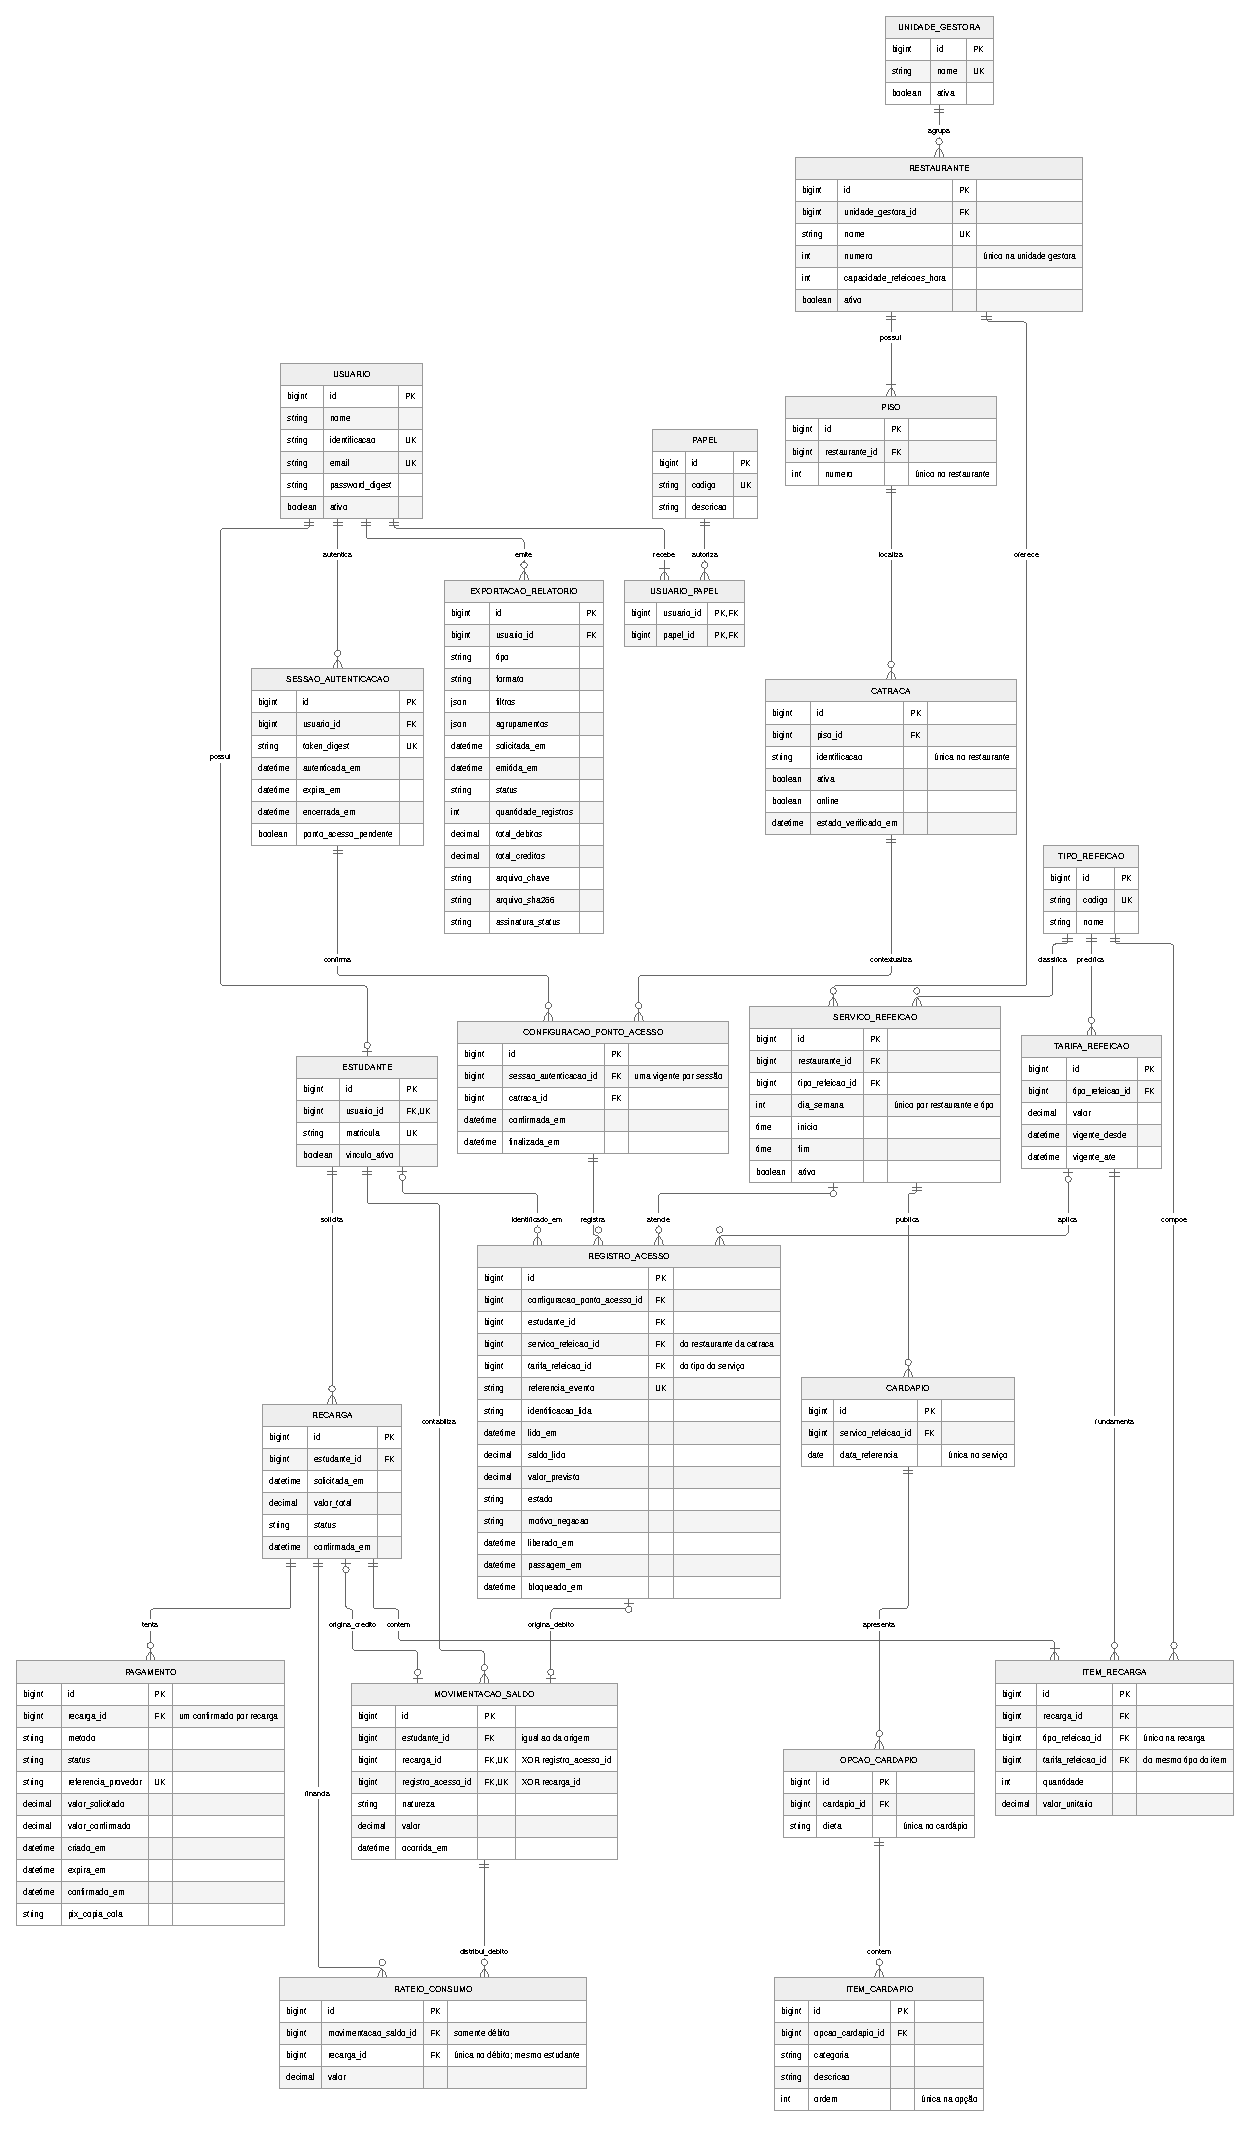
\includegraphics[width=\linewidth,height=0.88\textheight,keepaspectratio]{diagramas/visao-geral.pdf}
\end{center}
\clearpage

\clearpage
\subsection*{Visão 1 — Identidade e papéis}
\begin{center}
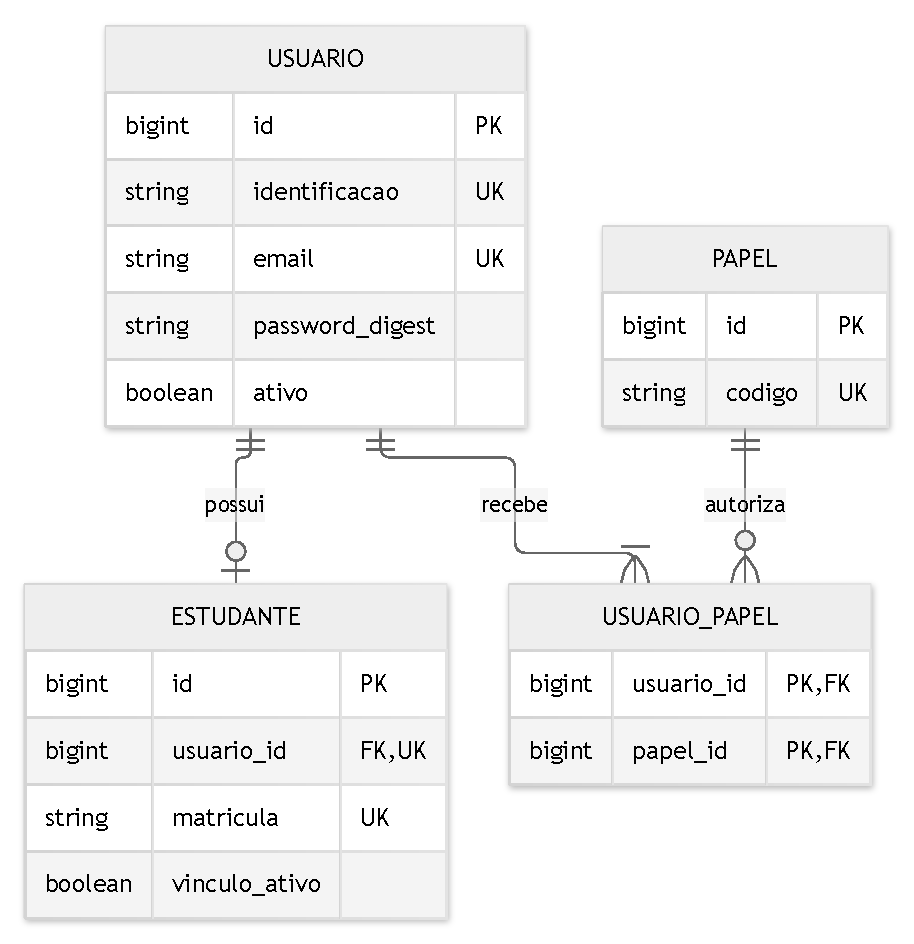
\includegraphics[width=\linewidth,height=0.88\textheight,keepaspectratio]{diagramas/visao-1.pdf}
\end{center}
\clearpage

\clearpage
\subsection*{Visão 2 — Sessão, ponto de acesso e emissão}
\begin{center}
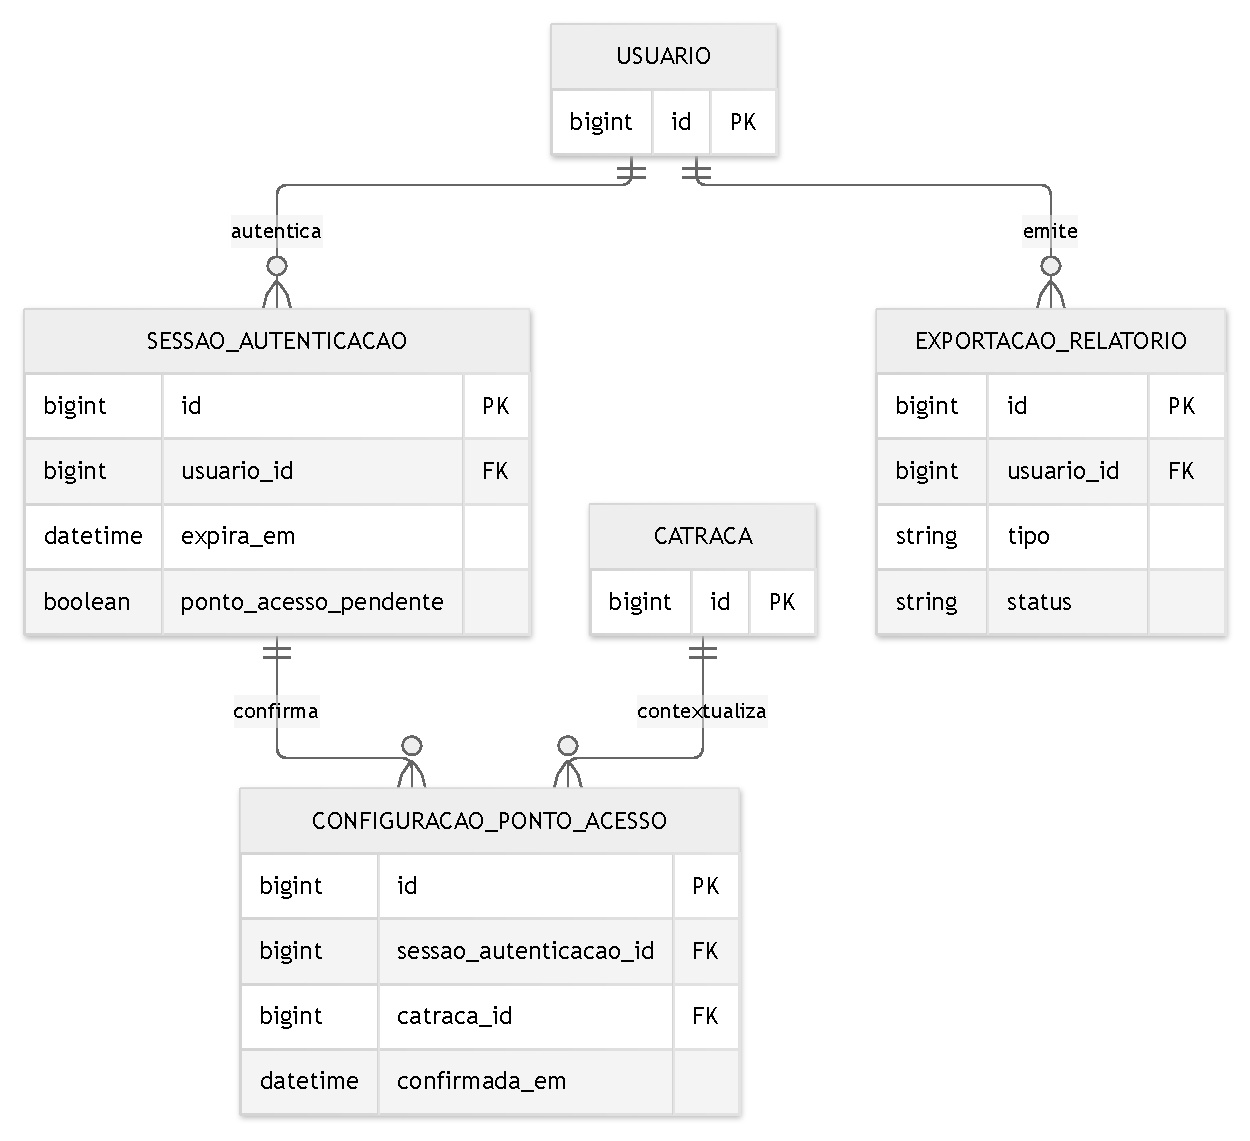
\includegraphics[width=\linewidth,height=0.88\textheight,keepaspectratio]{diagramas/visao-2.pdf}
\end{center}
\clearpage

\clearpage
\subsection*{Visão 3 — Estrutura física e oferta de refeições}
\begin{center}
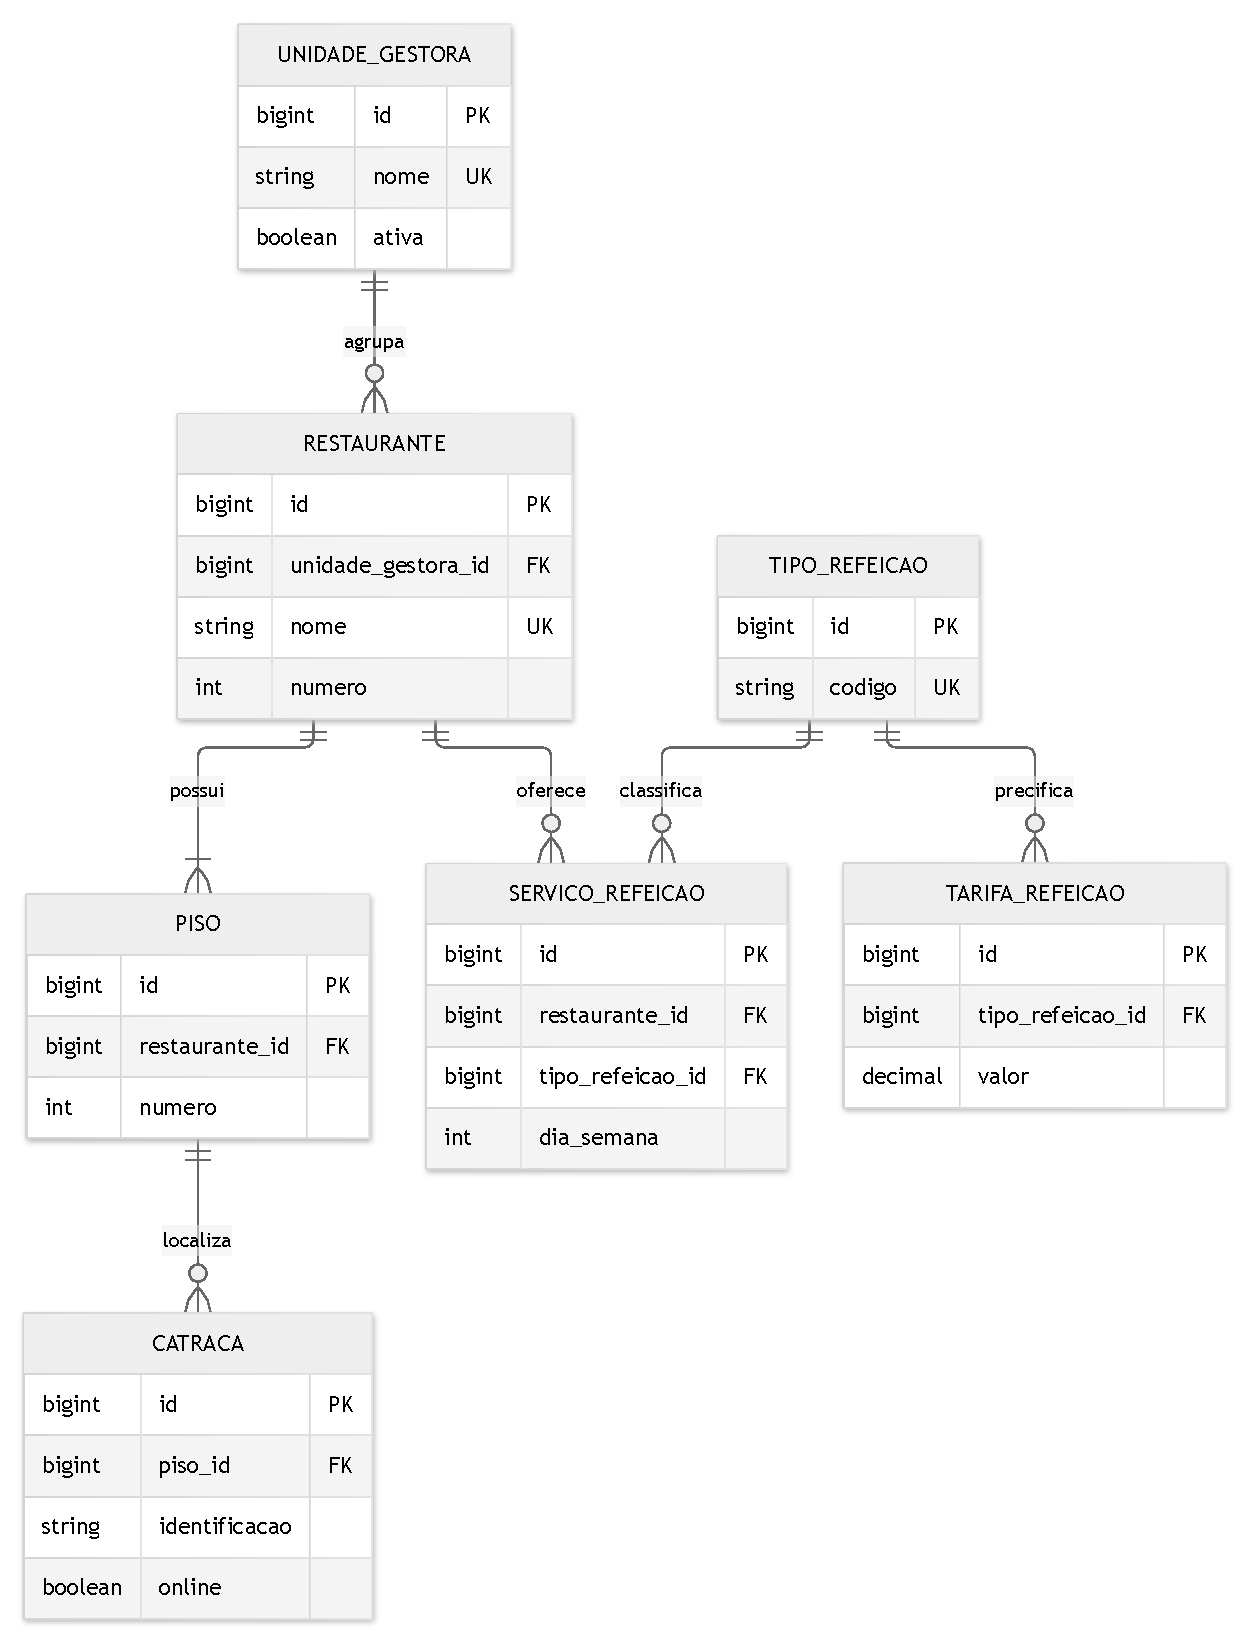
\includegraphics[width=\linewidth,height=0.88\textheight,keepaspectratio]{diagramas/visao-3.pdf}
\end{center}
\clearpage

\clearpage
\subsection*{Visão 4 — Compra e pagamento}
\begin{center}
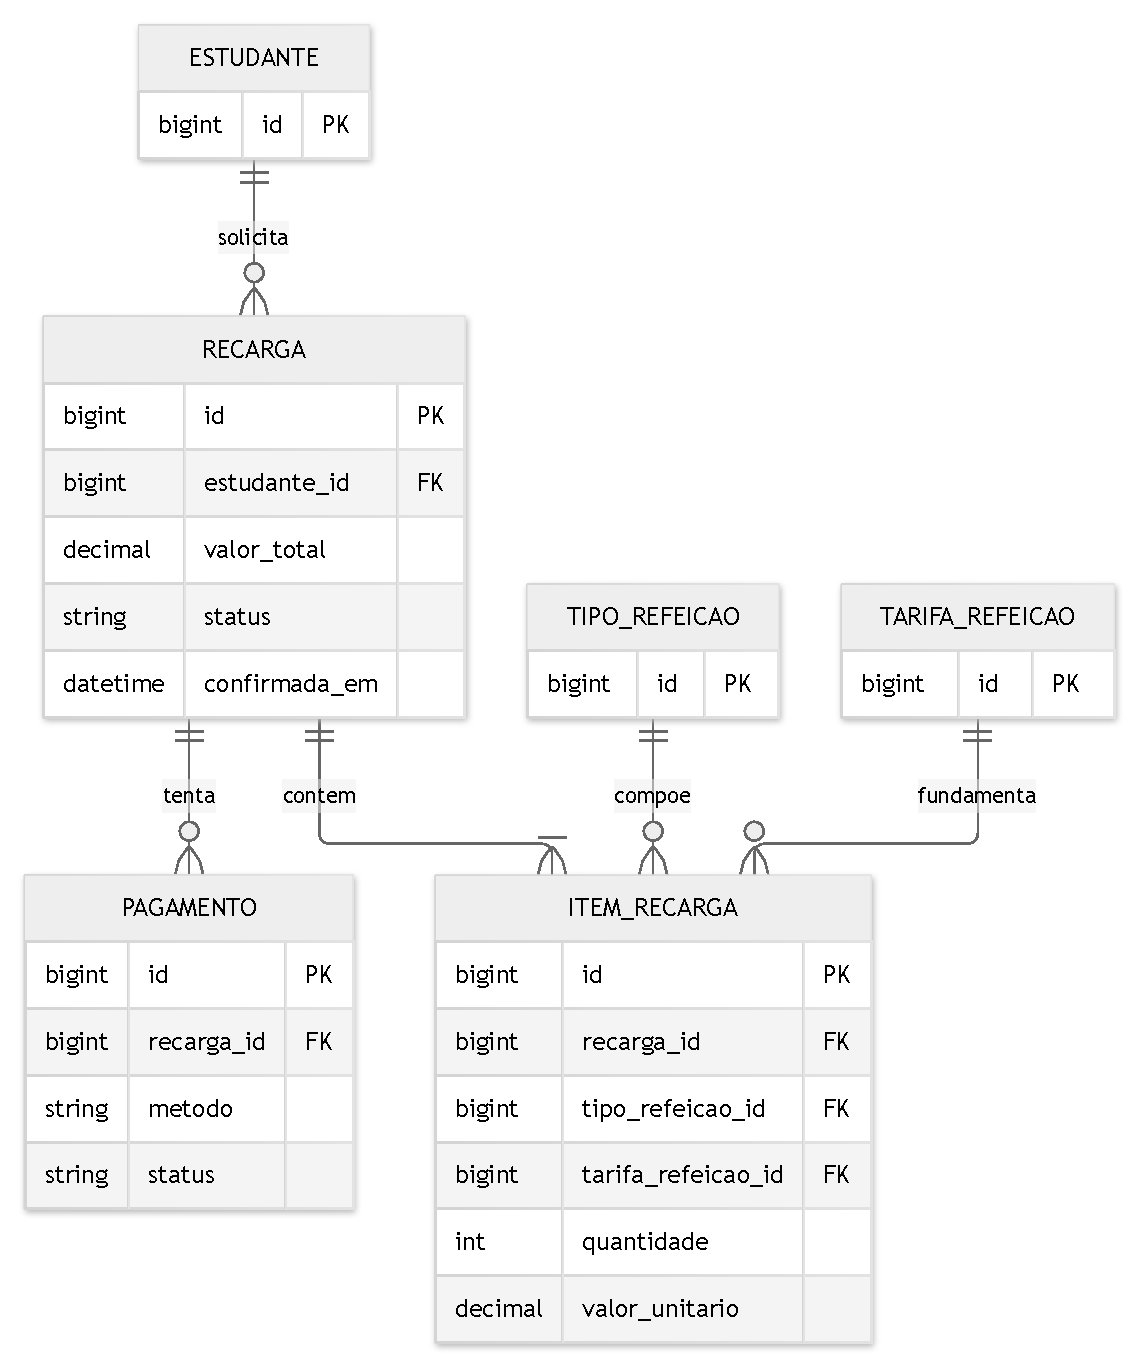
\includegraphics[width=\linewidth,height=0.88\textheight,keepaspectratio]{diagramas/visao-4.pdf}
\end{center}
\clearpage

\clearpage
\subsection*{Visão 5 — Extrato e origem dos recursos consumidos}
\begin{center}
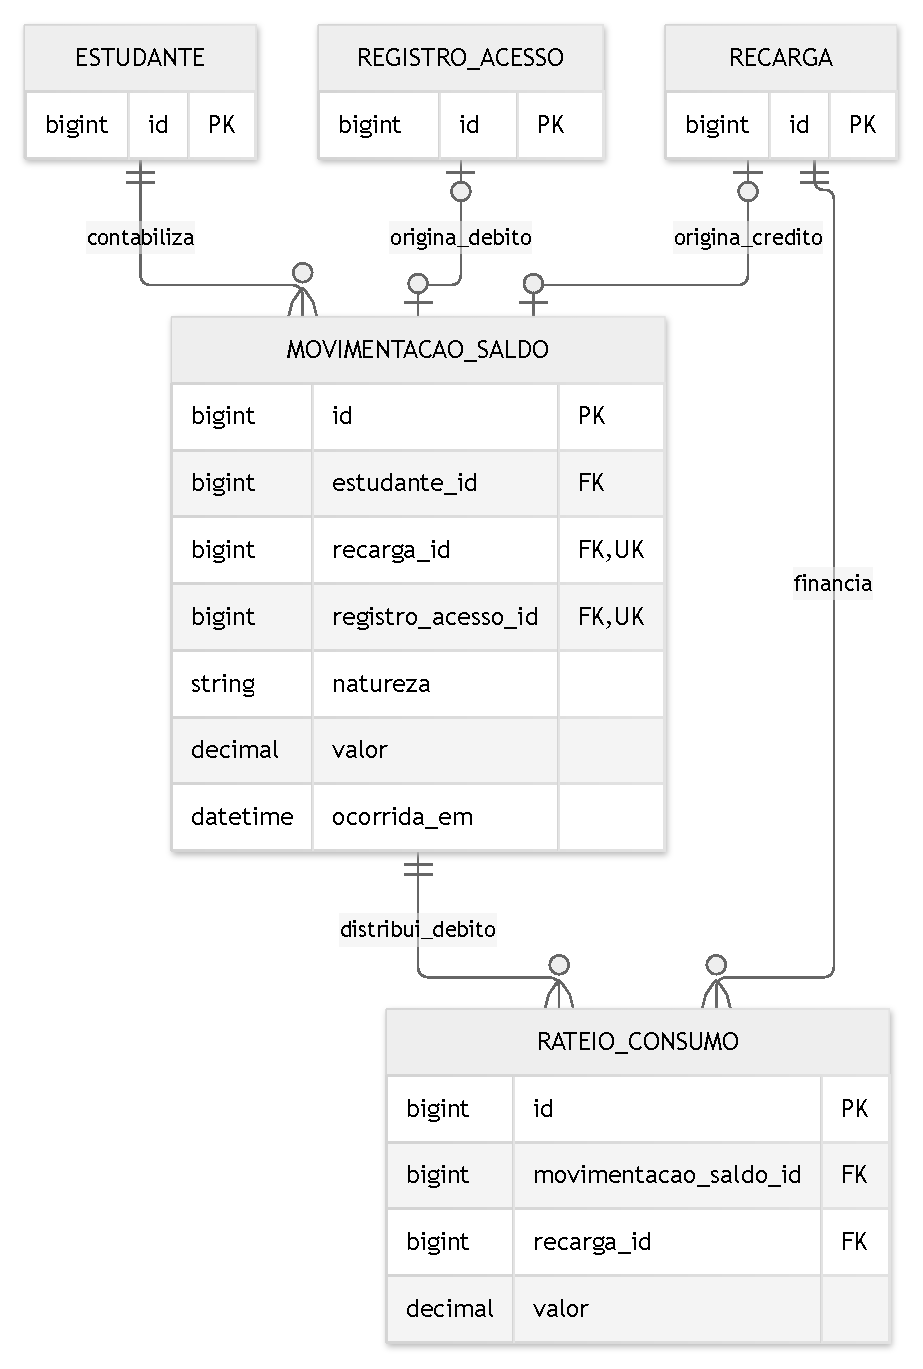
\includegraphics[width=\linewidth,height=0.88\textheight,keepaspectratio]{diagramas/visao-5.pdf}
\end{center}
\clearpage

\clearpage
\subsection*{Visão 6 — Leitura, autorização e passagem}
\begin{center}
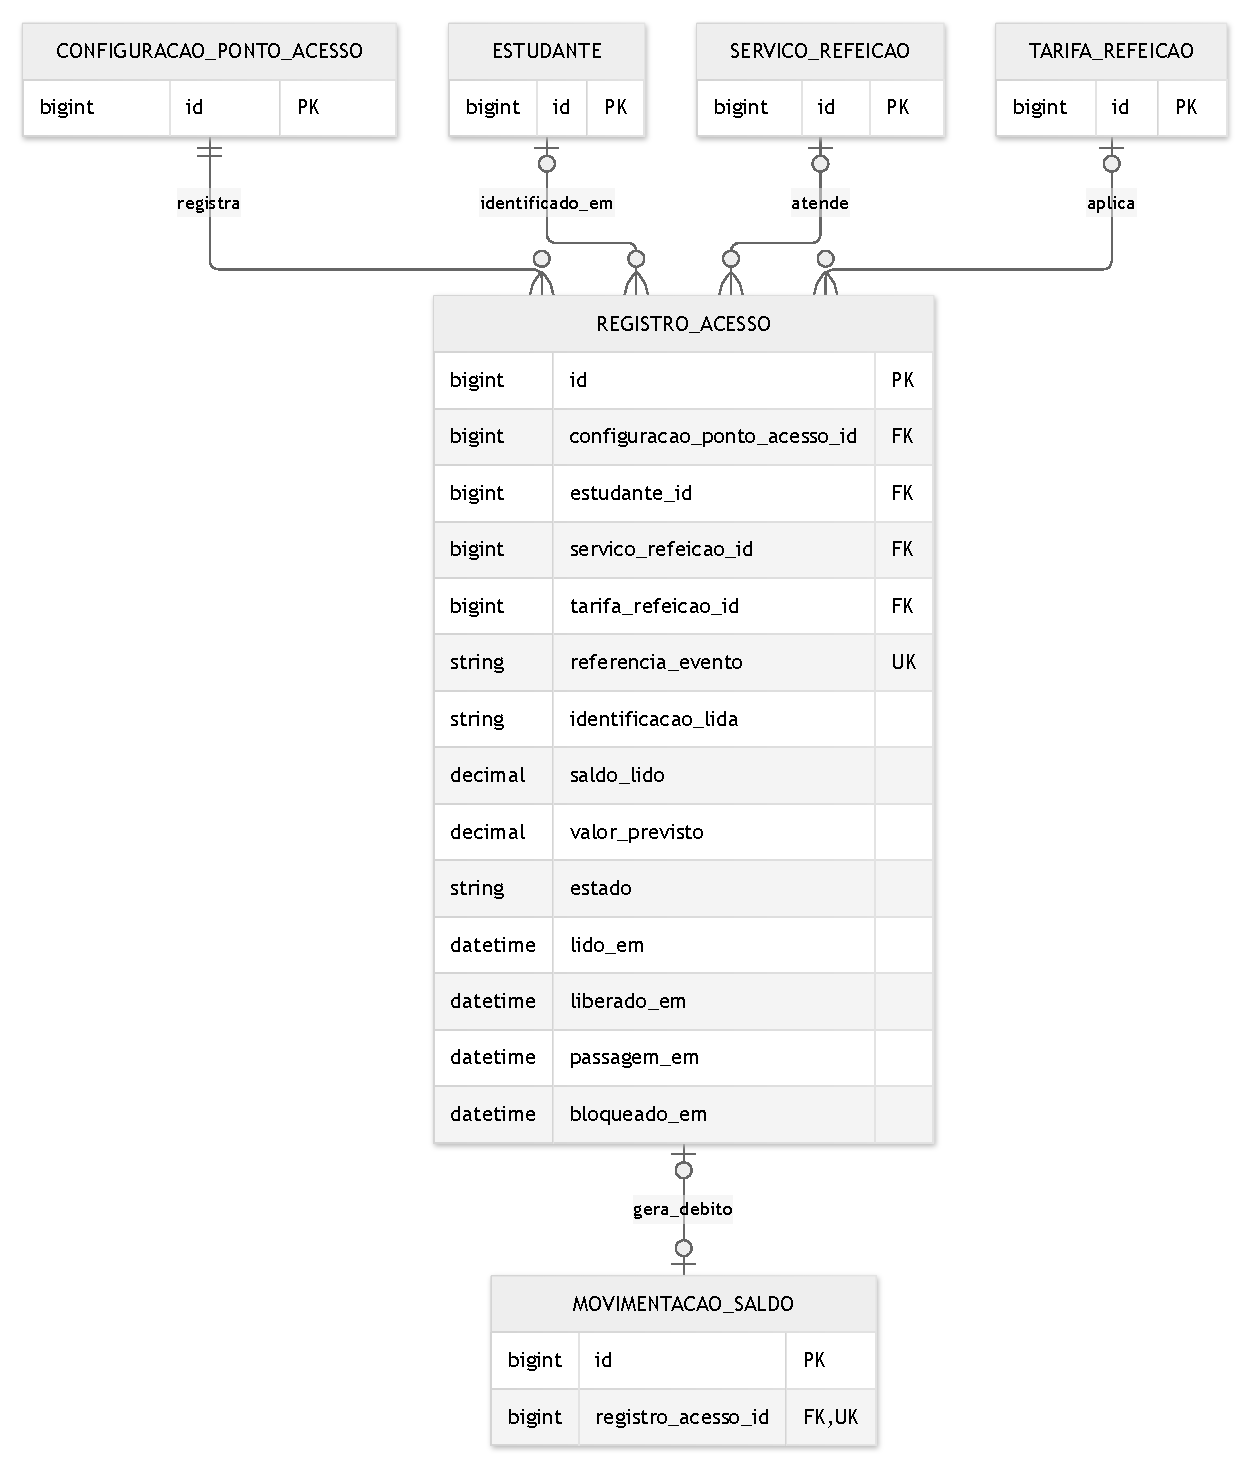
\includegraphics[width=\linewidth,height=0.88\textheight,keepaspectratio]{diagramas/visao-6.pdf}
\end{center}
\clearpage

\clearpage
\subsection*{Visão 7 — Cardápios e alternativas alimentares}
\begin{center}
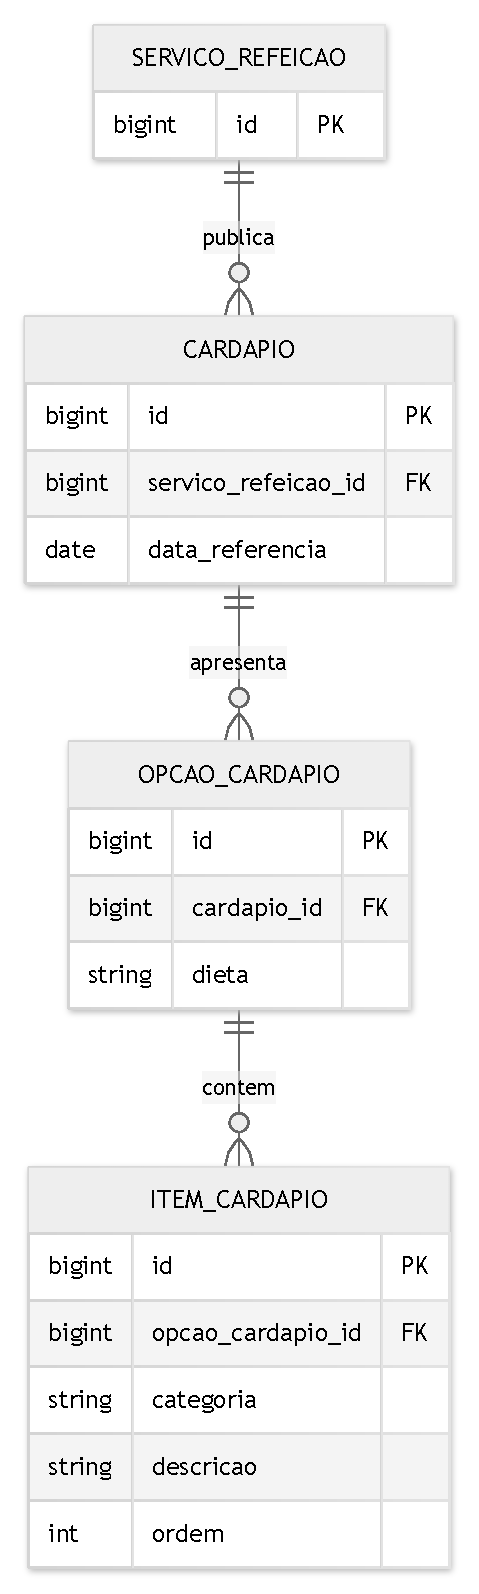
\includegraphics[width=\linewidth,height=0.88\textheight,keepaspectratio]{diagramas/visao-7.pdf}
\end{center}
\clearpage

\section{Considerações Finais}\label{considerauxe7uxf5es-finais}

O modelo cobre as 12 funcionalidades da primeira sprint com 23 entidades
e 30 relacionamentos, apresentados na visão geral e detalhados nas sete
visões parciais. Ao separar solicitação de recarga, confirmação de
pagamento, leitura na catraca e passagem efetiva, e ao registrar a
origem de cada lançamento, o esquema sustenta o extrato do estudante, o
histórico das catracas e os relatórios globais sem gerar créditos ou
débitos indevidos. Antes da implementação, o grupo ainda precisa definir
a política de tarifas, o critério de consumo dos créditos e o mecanismo
de assinatura digital dos relatórios.

\section{Apêndice --- Uso de inteligência
artificial}\label{apuxeandice-uso-de-inteliguxeancia-artificial}

Este relatório, sua proposta de modelo ER e os diagramas Mermaid foram
elaborados com apoio do \textbf{OpenAI Codex}. A estratégia utilizada
foi a leitura do enunciado e do template LaTeX fornecidos pelo usuário,
análise da wiki e dos 12 arquivos BDD, extração dos relacionamentos,
levantamento de restrições e comparação das regras entre
funcionalidades.

Foi utilizada a skill \textbf{plugin-management} para procurar uma
integração com Figma após a tentativa de leitura do protótipo pela web.
A integração não estava conectada durante a elaboração, portanto não se
afirma ter inspecionado os frames. Não foram utilizados agentes
paralelos. As entidades auxiliares e as decisões propostas estão
identificadas para que o grupo possa revisá-las e explicar sua
finalidade antes da entrega.

A visão geral do modelo foi elaborada posteriormente com apoio do
\textbf{Claude Code} (Anthropic, modelo Claude Opus 5.5), a pedido de um
integrante do grupo, que definiu a tarefa e revisou o resultado. A
estratégia foi a seguinte: a IA leu o dicionário de dados e as sete
visões, reuniu as 23 entidades com todos os atributos do dicionário e os
30 relacionamentos correspondentes às chaves estrangeiras, e eliminou um
relacionamento duplicado entre as visões 5 e 6, que representavam a
mesma chave estrangeira com rótulos diferentes. As anotações da última
coluna foram extraídas do dicionário e das regras de integridade do
relatório, sem acrescentar regras novas. Também não foram criadas chaves
estrangeiras deriváveis por outros caminhos.

A verificação foi automatizada por scripts auxiliares, que não fazem
parte do repositório. Um deles comparou o diagrama com o dicionário e
com as sete visões: entidades, atributos, chaves, obrigatoriedade e
unicidade das chaves estrangeiras e as cardinalidades resultantes. Esse
script foi testado com erros inseridos de propósito. Outro mediu a
legibilidade de 126 alternativas de layout do Mermaid, contando arestas
sobre marcadores de cardinalidade, sobre caixas ou sobre rótulos e
cruzamentos entre arestas; a alternativa adotada não apresenta os três
primeiros problemas e tem quatro cruzamentos. A IA ajustou ainda o
script \path|gerar_relatorio.py| para incluir a visão geral sem
renumerar as demais figuras, ajustar o PDF do diagrama a uma página e
manter a regra de quebra de identificadores longos independentemente dos
pacotes LaTeX instalados.

Na mesma ferramenta e a pedido do grupo, o relatório foi depois enxugado
para a entrega: foram retirados a seção de normalização e os apêndices
de integridade e de rastreabilidade, as considerações finais foram
condensadas em um parágrafo, e os apêndices do spike de views Rails e
das divergências entre cenários foram movidos, sem alteração, para o
arquivo \path|referencia-spike-views-e-decisoes.md|. Não foram
utilizados agentes paralelos.

\section{Referências}\label{referuxeancias}

\begin{itemize}
\tightlist
\item
  Enunciado da Sprint 1: \texttt{sprint1.pdf}, especialmente a seção
  ``Segunda etapa''.
\item
  Template fornecido:
  \path|TemplateRelatorioSprint1_1/ER-MyRottenPotatoes.tex|.
\item
  Wiki do projeto: \texttt{wiki/Home.md}.
\item
  Especificações de aceitação: os 12 arquivos em \texttt{features/}.
\item
  Dados de cardápio: \texttt{cardapio.json}.
\item
  Protótipo indicado no enunciado:
  \href{https://www.figma.com/design/Clozp7Rj1jOBz6l7LoT44t/UnB-RU---Engenharia-de-Software?node-id=0-1}{UnB
  RU no Figma}. Conteúdo visual não acessado.
\item
  \href{https://mermaid.js.org/syntax/entityRelationshipDiagram.html}{Mermaid
  --- Entity Relationship Diagrams}.
\end{itemize}

\end{document}
